\documentclass{beamer}
\usepackage[utf8]{inputenc}
%\usepackage[ngerman]{babel}
\usepackage{graphicx}
\usepackage{array}

\usetheme{Goettingen}
\begin{document}
    \section{Introduction}
        \begin{frame}
            \frametitle{Introduction}
            Population genetics aims to infer details of evolutionary processes based on the current population's genetic composition. \\
            Subfield of Genetics 
        \end{frame}

    \begin{frame}
        \frametitle{Single Nucleotide Variant(SNV)}
        \section{SNV}
        A single-nucleotide variant (SNV) is a variation in a single nucleotide that occurs at a specific position in the genome. This may be rare or common in a population. \\
    \end{frame}
    \begin{frame}
        \frametitle{Single Nucleotide Polymorphism(SNP)}
        \section{SNP}
        A single-nucleotide polymorphism (SNP) is a SNV that occurs in a significant proportion (typically $>$ 1\%) of a population. \\
        Polymorphisms describe sites (nucleotide positions, etc.) that are variable within a species; divergence describes sites variable between species.
        
    
    \end{frame}
    \begin{frame}
        \frametitle{Basic models of population growth}
        \section*{Population growth rate}
        $r = \frac{s(T)-s(T_0)}{s(T_0)}$ \\
        where s(T) is the population size at time T and s(T0) the size of the initial population at time T0. 
    \end{frame}
    \begin{frame}
        \frametitle{Alleles and ploidity}
        
        An allele is the variant form of a given gene found at the same chromosomal location.
        \\
        Ploidy is the number of sets of chromosomes in a cell and hence the number of possible alleles for genes.
    
        
    
    \end{frame}
    \begin{frame}
        \frametitle{Haploid and Diploid}
        \section*{Haploid and Diploid}
        Haploid Cells:
        Haploid cells have half the number of chromosomes (n) as diploid - germ cells Result of meiosis\\
        Example: sperm and egg cells\\
        Diploid Cells:
        Diploid cells contain two copies of each chromosome (2n) - somatic cells Result of mitosis\\
        Example: skin cells

    
        
    
    \end{frame}
    \begin{frame}
        \frametitle{Haploid Reproduction Model}
        \section*{Haploid Reproduction Model}
       - Assume constant population size\\
       - Each gene i in generation t + 1 is found by randomly choosing a predecessor gene g in generation t. This implies, that it is possible that one gene can have more than one offspring.\\
       - Any gene in generation t not chosen “dies out”.
        \begin{figure}
         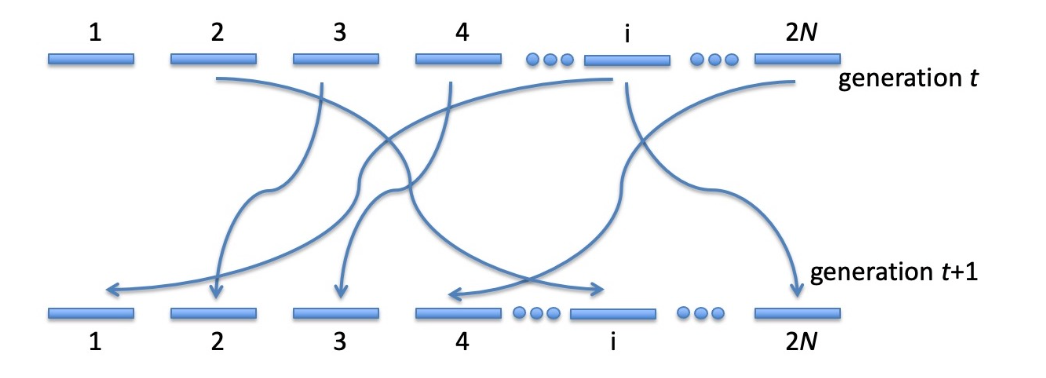
\includegraphics[width=\textwidth]{haploidRep.png}
            \caption{Haploid reproduction model}
        \end{figure}
 
    \end{frame}
    \begin{frame}
        \frametitle{Diploid populations}
        \section*{Diploid populations}
        Assumptions - 
        Species has 2 Sexes, Male ans Female. \\
        Each individual has 2 copies of each gene, a gene is chosen for each parent with equal odds \\
        In this model, each gene has one parent gene and each individual has two parents.\\
        For large values of N, Nf and Nm, one can approximate the diploid model by the haploid model.
        Thus, we will only consider the haploid model.\\
        \begin{figure}
            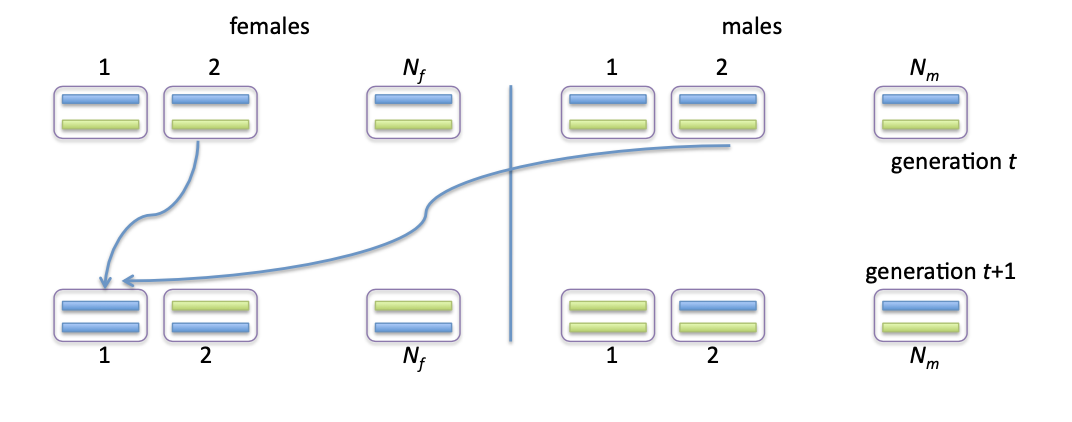
\includegraphics[width=0.8\textwidth]{diploidRep.png}
               \caption{Diploid reproduction model}
           \end{figure}

    
        
    
    \end{frame}
    \begin{frame}
        \frametitle{Haplotypes and Genotypes}
        \section*{Haplotypes and Genotypes}
        Haplotype: A haplotype is a sequence of an individual’s genome that occurs together on one or two homologous copies of a chromosome.\\
        Genotype: The two alleles at the same site on two homologous chromosomes form the genotype at that site. We denote that by ‘P$|$Q’, if ‘P’ and ‘Q’ are the alleles, respectively.
        Example \\
        An individual has the two haplotypes \\
        A T T G A C A T C \\
        A C T G A C A C T \\
        Then the genotype at the first site is A$|$A, at the second site T$|$C, and so on. \\
        Task- Show the full genotype of the individual.
    \end{frame}
    \begin{frame}
        \frametitle{Homozygous and Heterozygous}
        \section*{Homozygous and Heterozygous}

        A site c is called homozygous if the genotype consists of two identical alleles at c. The site c is called heterozygous if the genotype consists of two different alleles at c. \\
        Task- for an individual that has the two haplotypes \\
        A T T G A C A T C \\
        A C T G A C A C T \\
        give the set of homozygous and heterozygous sites. 
    
    \end{frame}
    \begin{frame}
        \frametitle{Most recent common ancestor(MRCA)}
        \section*{Most recent common ancestor(MRCA)}
        How many generations back is the most recent common ancestor (MRCA) of two present-day genes?
        
    
    \end{frame}
    \begin{frame}
        \frametitle{Wright Fisher Model}
        \section*{Wright Fisher Model}
        Key assumptions of the Wright-Fisher model: \\
        1. Discrete and non overlapping generations. \\
        2. Constant population size. \\
        3. Haploid individuals \\
        4. All individuals are equally fit. \\
        5. The population has no geographic or social structure\\
        6. No recombinations of genes (or sequences)



    
        
    
    \end{frame}
\end{document}
